\documentclass{article}
\usepackage{graphicx}
\usepackage[utf8]{inputenc}
\usepackage{amsmath, amssymb, latexsym}

\usepackage{pgfplots}
\usepackage{algorithm}
\usepackage[noend]{algpseudocode}
\usepackage{tikz}
\usepackage{nicefrac}
\pgfplotsset{every axis legend/.append style={
at={(0,0)},
anchor=north east}}
\usetikzlibrary{shapes,positioning,intersections,quotes}
\usetikzlibrary{arrows.meta,
                bending,
                intersections,
                quotes,
                shapes.geometric}
                
\definecolor{darkgreen}{rgb}{0.0, 0.6, 0.0}
\definecolor{darkred}{rgb}{0.7, 0.0, 0.0}
\makeatletter
\makeatother
\begin{document}

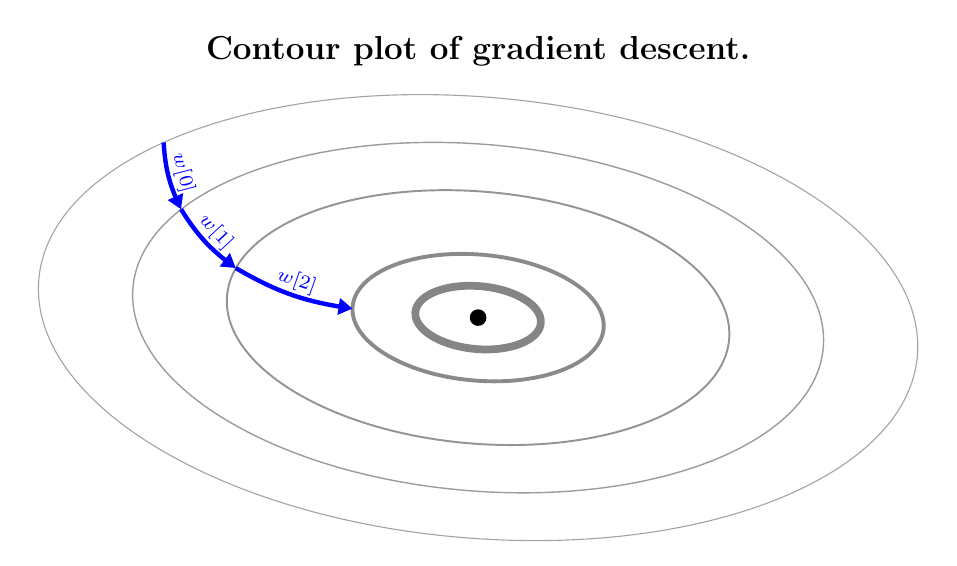
\begin{tikzpicture}[
  every edge/.style = {draw, -{Triangle[angle=60:1pt 3,flex]},
  bend right=11, blue,ultra thick},
  every edge quotes/.style = {font=\scriptsize, inner sep=1pt,
      auto, sloped}
  ]
  \fill (0,0) circle[radius=3pt];
  \path[name path=C] foreach \i in {4, 8, 16, 22, 28}
    {(0,0) circle[draw=red!\i, x radius=2*\i mm, y radius=\i mm, rotate=-5]};
  \foreach \i in  {4, 8, 16, 22, 28}
  \draw[line width=11.2/\i, draw=white!\i!gray]
  (0,0) circle[x radius=2*\i mm, y radius=\i mm, rotate=-5];
  \path[name path=V] (-4,2.4) .. controls + (0,-2) and + (-2,0) .. (0,0);
  %
  \draw [name intersections={of=C and V, sort by=C, name=A}]
  (A-5) edge ["${w[0]}$"] (A-4)
  (A-4) edge ["${w[1]}$"] (A-3)
  (A-3) edge ["${w[2]}$"] (A-2);
  \node[above,font=\large\bfseries] at (current bounding box.north) {Contour plot of gradient descent.};
\end{tikzpicture}


\end{document}